\documentclass{article}

\usepackage[utf8]{inputenc}
\usepackage[english]{babel}
\usepackage{blindtext}
\usepackage{graphicx}
\usepackage{amsmath}
\usepackage{float}
\usepackage[compact]{titlesec}
\usepackage{multicol}
\usepackage[a4paper, total={7.5in, 10in}]{geometry}

\usepackage{listings}
\usepackage{color}
 
\definecolor{codegreen}{rgb}{0,0.6,0}
\definecolor{codegray}{rgb}{0.5,0.5,0.5}
\definecolor{codepurple}{rgb}{0.58,0,0.82}
\definecolor{backcolour}{rgb}{0.95,0.95,0.92}
 
\lstdefinestyle{mystyle}{
    backgroundcolor=\color{backcolour},   
    commentstyle=\color{codegreen},
    keywordstyle=\color{magenta},
    numberstyle=\tiny\color{codegray},
    stringstyle=\color{codepurple},
    basicstyle=\footnotesize,
    breakatwhitespace=false,         
    breaklines=true,                 
    captionpos=b,                    
    keepspaces=true,                 
    numbers=left,                    
    numbersep=5pt,                  
    showspaces=false,                
    showstringspaces=false,
    showtabs=false,                  
    tabsize=2
}
 
\lstset{style=mystyle}

\setlength{\columnsep}{1cm}
\setlength{\parindent}{0em}
\titlespacing{\section}{1pt}{*0.5}{*0.5}

\begin{document}

\textbf{Relatório de Entrega de Trabalho} \newline
\textbf{Disciplina de Programação Paralela (PP)}\textbf{ - Prof. César De Rose} \newline
\textbf{Alunos:} Rafael Rios e Rodrigo Silveira \newline
\textbf{Exercício:} TPD2: Algoritmos Distribuídos de Eleição (MPI) \newline

\begin{multicols*}{2}

\section{Modelagem utilizada}
A fim de avaliar a execução de um algoritmo de distribuição por eleição, usou-se a biblioteca MPI (Message Passing Interface), a qual implementa diversas funções que compreendem um padrão para comunicação de dados em computação paralela, para desenvolver a modelagem de um anel lógico para 'n' processos. Desta forma, o anel deve trocar mensagens apenas com o próximo nodo seguinte a ele, onde o processo de maior índice corresponde ao coordenador. O sistema de eleição é proposto quando o coordenador falha, neste caso, um dos processos deve avisar os demais que uma eleição para a escolha do próximo coordenador ocorrerá. \newline


\section{Implementação}

o processo que detecta falha espera todos do anel receberem que é ele que vai detectar, para nao ter problemas de sincronização.


\section{Dificuldades encontradas}
avisar a todos quem vai detectar a falha pq se agente chamasse rand em todos os processos tipo, um processo tem que chamar rand e propagar para todos os outros.


\section{Testes}
Foram executados testes para diversos números de processos diferentes, visando observar possíveis falhas e mudanças no desempenho, para todas as execuções obteve-se o mesmo resultado esperado, como também, o mesmo desempenho.


\section{Observações Finais}



\end{multicols*}

\newpage

\lstinputlisting[language=C++]{pipe_basico.c}

\newpage

\begin{figure}[H]
            \centering
            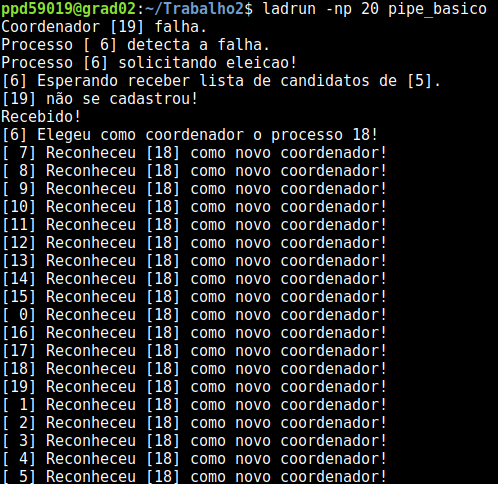
\includegraphics[width=13cm, height=12cm]{exemplo_saida.png}
            \caption{Saída com 20 processos}
\end{figure}

\begin{figure}[H]
            \centering
            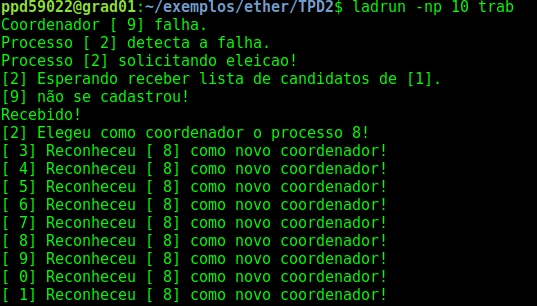
\includegraphics[width=13cm, height=8cm]{ex_10.png}
            \caption{Saída com 10 processos}
\end{figure}

\end{document}
